% !TEX root = ../main.tex

\chapter{Experiments}
\label{ch:experiments}
The goal of this chapter is to try to get closer to understand how much the ideas presented in the previous chapters could potentially benefit a concrete setup and implementation in the real world. As already quite extensively discussed in section \ref{sect:rmionbmv2:evaluation} the P4 implementation as is cannot be tested on real world hardware. With this in mind the first section of this chapter will explain the chosen approach to still try to measure something useful in order to evaluate the potential impact. Further, section \ref{sect:experiments:results} will present the measured results on the test university machine and finally the last section of this chapter will once again try to put the measured results into perspective and give an evaluation.

\section{Method}
\label{sect:experiments:methods}
As previously stated the following method was chosen since not being able to actually run the generated P4 source code on concrete real world hardware due to multiple reasons also already discussed previously. In order to come up with some alternative we started with the idea that instead of actually measuring lookup time on concrete network hardware we could instead measure the pure lookup time in an existing implementation and go on from there. We would use what we measured as maximally possible speed up. This immediately leads to the already established separation between pure lookup operation time and time spent for the last mile search. For this having the SOSD benchmark that can precisely measure the time it takes for a specific amount of lookups including last mile search on a dataset comes in handy. In order to measure hypothetical maximal time gain it is enough to separate the last mile search and measure only the pure lookup time. The final piece to the puzzle now is that we have to assume that our network switches are able to process packets at a higher or at least a similar rate than a processor can handle last mile searches. This initially seemed like a bold claim to me but when taking into account that switches usually operate at extremely high speed and that the proposed RMI implementation in P4 can easily scale horizontally with the amount of network hardware available, this quickly becomes realistic. Finally if we wanted to look at a closed system and effectively evaluate which method is faster, we would have to consider round trip time of packets. Since not even being able to reliably test any of the implementation on actual hardware, this major concern for a real world setup is neglected in the scope of this work. In that sense we assume an application where packets need to travel over the network and with that over a P4 capable network switch anyways. This leads to travel time spent not really being lost, but instead being used more efficiently.

\section{Results}
\label{sect:experiments:results}

\subsection{Individually measuring pure lookup and last mile search time}
In order to perform these measures we adapted the existing SOSD benchmark to measure not only lookup time and last mile search times at the same time but instead differenciate between the two steps and measuring only one at a time. The initial result though, when measuring only pure lookup operation time, is very disappointing. As shown in figure \ref{fig:books_200M_uint32-no-cc-mf} only a very small amount of time is spent on performing the pure RMI lookup operations.

\captionsetup[figure]{skip=10pt} % move caption down
\begin{figure}[!ht]
  \centering
  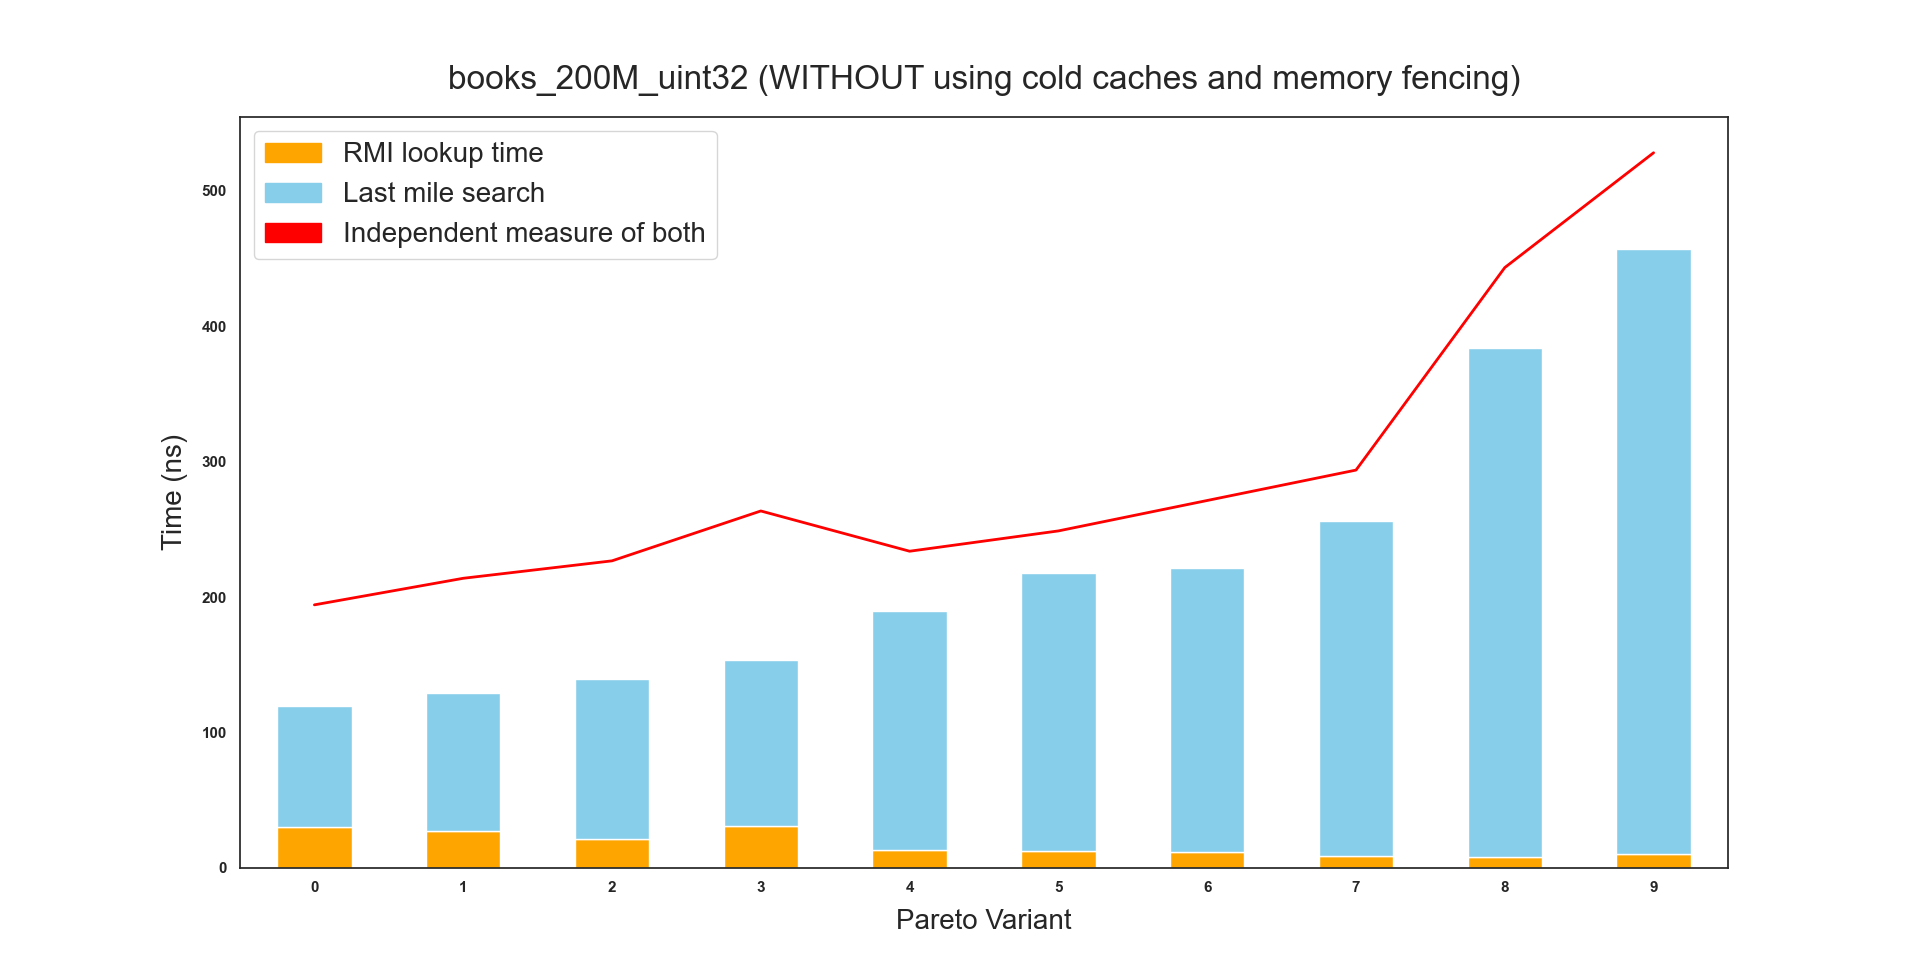
\includegraphics[width=1\textwidth]{measurements/books_200M_uint32-no-cc-mf}
  \caption[Lookup and last mile search time measures \emph{without using} cold caches and memory fencing]{
    Running the SOSD benchmark on the \emph{books\_200M\_uint32} dataset \emph{without using} cold caches or memory fencing, differentiating between pure lookup time and last mile search time.
  }
  \label{fig:books_200M_uint32-no-cc-mf}
\end{figure}

There are reasons for the way these measurements turned out which were already pointed out in section 4.4 of \cite{sosd-vldb}. Namely these reasons are that lookups in a tight loop can greatly benefit from low level CPU optimization techniques like operator reordering or caching. The same applies for the measurements in the figure above in an even more intense way, since only measuring performance of essentially lots of tightly repeated FMA instructions which the processor will optimize into a more optimal instruction order and therefore exaggerate the measured performance. The same holds true for caching, in the sense that some of the requested data will already be loaded in some cache level and therefore access time is greatly reduced.

\subsection{Using cold caches and memory fencing}
Luckily the authors of \cite{sosd-neurips} suggest and also implemented a way to mitigate these usually very desired CPU optimizations in the SOSD benchmark. The two proposed techniques aim at starting from a fresh CPU state before every lookup calculation. The first technique called cold caching mitigates cache side effects by filling the L3 CPU cache with a constant randomly generated set of numbers before each lookup. The second technique called memory fencing aims at mitigating instruction reordering by introducing memory fences before each lookup using the appropriate CPU instruction. With these techniques in place running SOSD takes a lot longer and RMI performance drastically decreases but with the advantage that more reliable meaures can be taken. The results from running the SOSD benchmark on the same dataset as previously but now using cold caches and memory fencing are shown in figure \ref{fig:books_200M_uint32}. Very similar observations can be made for all remaining 64-bit datasets provided by the SOSD benchmark shown in the appendix in section \ref{sect:appendix:measurements}.

\captionsetup[figure]{skip=10pt} % move caption down
\begin{figure}[!ht]
  \centering
  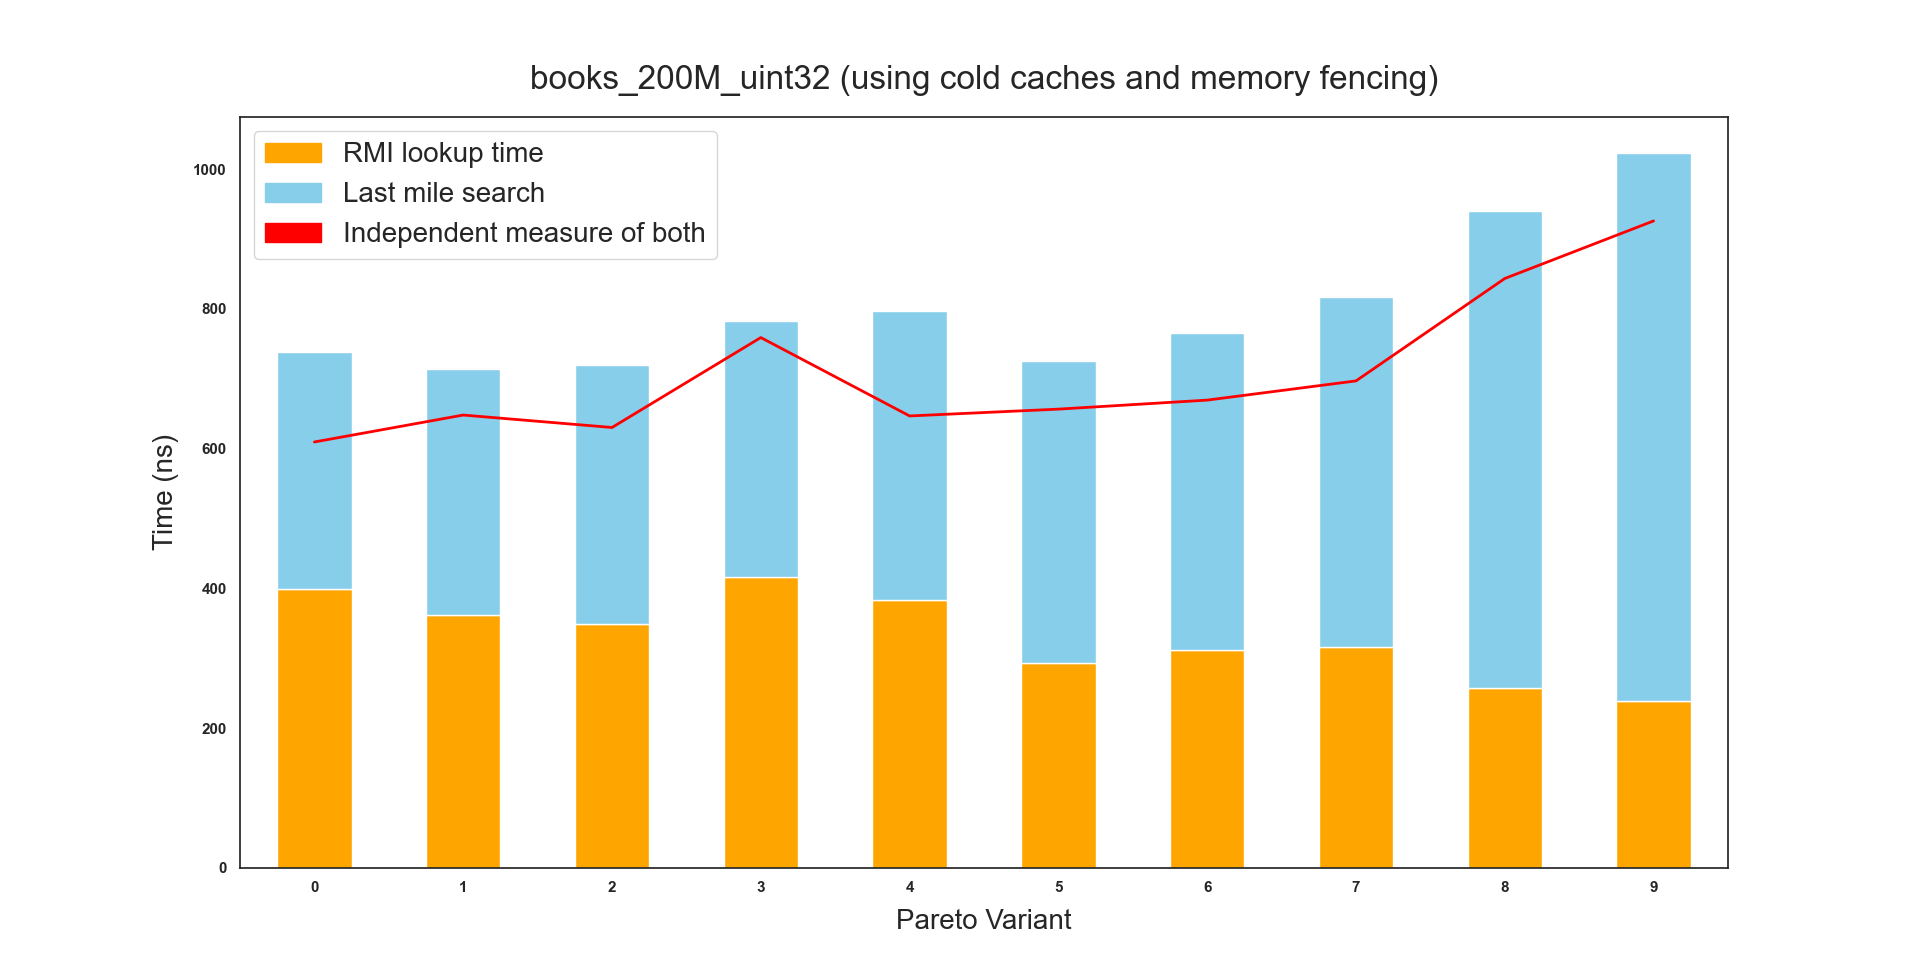
\includegraphics[width=1\textwidth]{measurements/books_200M_uint32}
  \caption[Lookup and last mile search time measures \emph{using} cold caches and memory fencing]{
    Running the SOSD benchmark on the \emph{books\_200M\_uint32} dataset \emph{using} cold caches and memory fencing, differentiating between pure lookup time and last mile search time.
  }
  \label{fig:books_200M_uint32}
\end{figure}

\subsection{Roughly approximating pure lookup time by the difference of total and last mile search time}
Finally the observation which probably leads to the best approximation of how long the pure RMI lookup operations actually take without cold caches and memory fencing, is when taking a normal measure (the red line in figure \ref{fig:books_200M_uint32-no-cc-mf}) and subtracting the last mile search time from this measure in order to guess the pure lookup operation time. This makes sense under the assumption that the last mile search code is less affected by operation reordering and caching. This is then visualized in figure \ref{fig:books_200M_uint32-no-lookup}. As for the previous experiment, similar graphs can be plotted for the remaining 64-bit datasets provided by the SOSD benchmark shown in the appendix in section \ref{sect:appendix:measurements-no-lookup}.

\captionsetup[figure]{skip=10pt} % move caption down
\begin{figure}[!ht]
  \centering
  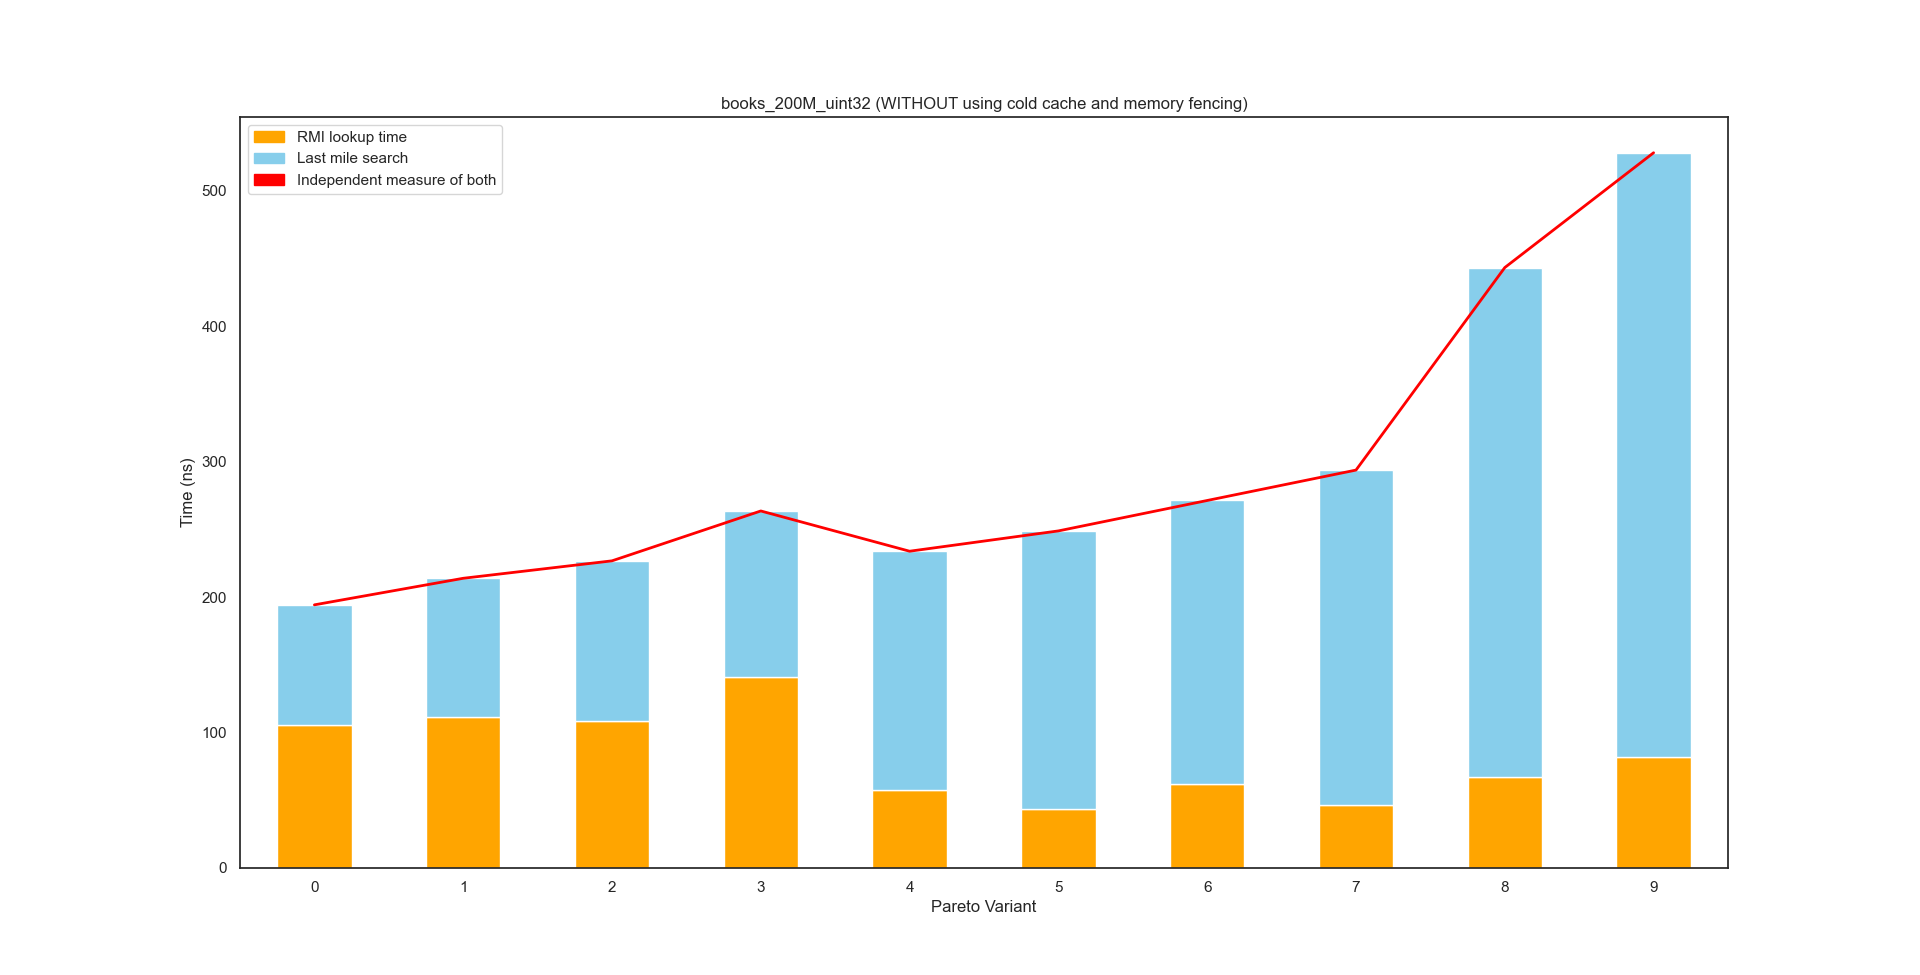
\includegraphics[width=1\textwidth]{measurements/books_200M_uint32-no-lookup}
  \caption[Last mile search time measures and lookup time approximation \emph{without using} cold caches and memory fencing]{
    Running the SOSD benchmark on the \emph{books\_200M\_uint32} dataset \emph{without using} cold caches and memory fencing, trying to approximate pure lookup time by subtracting the last mile search time from the independently measured total time.
  }
  \label{fig:books_200M_uint32-no-lookup}
\end{figure}

\subsection{Experiment observations}
When looking at the experiment figures, one can observe that the height of the blue bar (representing the last mile search time) increases with increasing pareto variant. This is expected since the SOSD benchmark trains its RMIs with decreasing index size limit relative to increasing pareto variant, meaning that with decreasing index size the last mile search bound becomes larger and therefore time spent to find a key in said larger bound increases. A next observation which is pointed out in \cite{sosd-vldb} is that the intensity at which RMI benefits from low level CPU optimizations heavily depends on many factors such as the shape of the data itself and the actual optimization capability of the processor doing the calculations. This forcibly means that any measure becomes very heavily application dependant and therefore the best advice is still to test different (learned) indexing algorithms individually in concrete applications. Still, a regular CPU can highly improve RMI performance in practice, while switches do not currently support any sort of CPU optimization techniques at this level. Concretely this means that it makes sense to compare measures from figure \ref{fig:books_200M_uint32} without any CPU optimizations at play, when directly trying to compare a server's RMI lookup performance against a switch's RMI lookup performance. Due to reasons already pointed out multiple times, this comparision is unfortunately currently not possible in practice. On the other hand, when opting for a comparision under ideal conditions, we can refer to figure \ref{fig:books_200M_uint32-no-lookup}, especially if we want to know how fast our university machine can handle last mile searches only.

\section{Evaluation}
After having described our measurement method in the first section and showing visualized results in the previous section, this section focuses on giving potential take-aways from what we measured and showing that outsourcing a learned index structure to the network can lead to a speed up. The major drawback that this work makes apparant is that there are lots of requirements currently missing in real world hardware. Namely these consist of what has been described in section \ref{sect:rmionbmv2:evaluation}.\\

Our university machine's CPU takes around 80 - 400ns for a full RMI lookup, including pure lookup operations as well as last mile search, without cold caches and memory fences (Refering to figure \ref{fig:sosd_lookups}). This means that our machine can handle between 2.5 - 12.5 million full RMI lookups per second. When now looking at the graphs in figure \ref{fig:books_200M_uint32-no-lookup} and section \ref{sect:appendix:measurements-no-lookup} we find that the pure RMI lookup calculations take pretty constantly around 50 - 100ns depending on the RMI layer configuration. Further, our university machine which would only have to deal with last mile searches and could outsource the pure lookup calculations to the switch could handle between 3 - 20 million last mile searches per second and takes around 50 - 300ns for a single last mile search.\\

All in all we find that by outsourcing the RMI calculations to the switch we can constantly gain around 50 - 100ns per lookup depending on the RMI configuration but independently of the RMI's index size and with that it's last mile search bound size, which means that without performing the RMI lookup calculations a server can constantly handle more lookups per second (since the server only has to perform the last mile searches). Further, if only a single Intel® Tofino™ 3 switch can provide pure lookup operations at a rate of around 10 billion packets per second \cite{tofino3-brief}, then this switch would easily outperform multiple magnitudes of servers working on last mile searches. This means that in a closed system the amount of speed gained, when outsourcing RMI to the network, is determined by the amount of last mile search workers. Each of them can treat more last mile searches per second and adds to the overall speed up. Additionally the constantly less time not spent on the server for calculating pure lookups would be mostly free, especially when having an application in mind where a lookup has to be sent over the network anyways. Finally, when reaching a point where a single switch cannot outperform all of the available last mile search workers anymore, horizontal scaling in terms of network switches is perfectly compatible with our RMI implementation in P4.\\
